% @author: MetaboHUB
% @date: 2014/10/20
% @note: this document is versioned through a GIT repository; sharing is caring

\documentclass[a4paper,11pt]{article}

%%%%%%%%%%%%%%%%%%%
% Polices 
\renewcommand*\sfdefault{cmss}
\renewcommand*\familydefault{\sfdefault}  %% Only if the base font of the document is to be sans serif

%%%%%%%%%%%%%%%%%%%
% packages
\usepackage{cmbright}
\usepackage{algorithm}
\usepackage{algorithmic}
\usepackage{amssymb}
\usepackage{amsmath}
\usepackage{pifont}
\usepackage[usenames,dvipsnames]{color}

\usepackage{wallpaper}
\usepackage[utf8]{inputenc} % accents
\usepackage[english]{babel}
\usepackage{fixltx2e}

\usepackage{array}
\usepackage{color}

% margins
\usepackage{geometry}
\geometry{left=2.3cm,right=2.3cm,top=3cm,bottom=2cm}

% pdf hyperlinks
\usepackage{hyperref}

%%%%%%%%%%%%%%%%%%%%%%%%%%%%%%%%%%%%%%%%%%%%%%%%%%%%%%%%%%%%%%%%%%%%% metadata
\usepackage{hyperref}
\hypersetup{
	pdftitle={Spectral Database - WebApp Installation Documentation},
	pdfauthor={MetaboHUB - WP3},
	colorlinks=true,
	urlcolor=blue,
	linkcolor=black,
	citecolor=black,
}

% dates
\usepackage{datetime}
\usepackage{multirow}
\usepackage{tabularx}
\usepackage{hyperref}
\usepackage{pifont}

% italic text
\newcommand{\ie}{\textit{i.e.}~}
\newcommand{\eg}{\textit{e.g.}~}
%\newcommand{\exp}{\textit{exp}~}
\newcommand{\cf}{\textit{cf.~}}
\newcommand{\textitt}[1]{\textit{\texttt{#1}}}
\def\myversion{0.1}

%tickmarks
\newcommand{\tick}{\textcolor{ForestGreen}{\ding{52}}}
\newcommand{\tickNo}{\hspace{1pt}\textcolor{BrickRed}{\ding{55}}}

%colors
%\usepackage[table]{xcolor}
\definecolor{inraGreen}{rgb}{0.50196078431,0.62745098039,0}
\definecolor{mthRed}{rgb}{1,0.00784313725,0.00784313725}
%%%%%%%%%%%%%%%%%%%

% meta-data
\author{MetaboHUB - WP3}
\date{2014}

%%%%%%%%%%%%%%%%%%%
% title page 
\newcommand{\HRule}{\rule{\linewidth}{0.5mm}}

% version
\input{vc.tex}

\begin{document}
%%%%%%%%%%%%%%%%%%%%%%%%%%%%%%%%%%%%%%%%%%%%%%%%%%%%%%%%%%%%%%%%%%%%% title page
% @author: MetaboHUB
% @date: 2014/02/20
% @note: this document is versioned through a GIT repository; sharing is caring

\begin{titlepage}

\begin{center}

% Upper part of the page

\includegraphics[width=0.7\textwidth]{./files/images/mth_title.jpg}\\[1cm] 

% Title
\HRule \\[0.4cm]
\begin{center} { \textsc{\large { \huge \bfseries \colorbox{Black}{\color{White}Metabo{\color{mthRed}HUB}} WP3 \\}} } \end{center} %\\[0.4cm]
\begin{center} { \textsc{\large { \huge \bfseries Spectral Database}} } \end{center} %\\[0.4cm]
\begin{center} { \huge \bfseries Peak Forest Install Guide - v 1.0} \end{center} 

%{ \huge \bfseries }\\[0.4cm]
\HRule \\[0.4cm]

 \large Peak Forest: Documentation for deployment.

\HRule \\[1.5cm]

% Author and date
\begin{flushleft}
 \large
Author: Nils Paulhe \\[\baselineskip]
Validator: Franck Giacomoni \\[\baselineskip]
Date: \today

% version
\let\thefootnote\relax
\footnotetext{Base revision~\GITAbrHash, \GITAuthorDate, \GITAuthorName.}

\end{flushleft}

\vfill

\end{center}

\end{titlepage}

%% version
%\let\thefootnote\relax
%\footnotetext{Base revision~\GITAbrHash, \GITAuthorDate, \GITAuthorName.}

% logo on corener
%\ULCornerWallPaper{0.30}{files/xxx.jpg}
\URCornerWallPaper{0.20}{files/images/logo_mth.png}
%%%%%%%%%%%%%%%%%%%

\tableofcontents

\listoffigures


\newpage

%%%%%%%%%%%%%%%%%%%%%%%%%%%%%%%%%%%%%%%%%%%%%%%%%%%%%%%%%%%%%%%%%%%%% START

% \section{Document History} % keep commented
% \begin{itemize}
% 	\item 2014/10/20: v 0.1~: document template (init; main sections).
% \end{itemize} 

\section{Introduction}
\subsection{About}
As a part of the MetaboHUB project, the Peak Forest web-application is integrated in the Spectral Database project. 
This web-application provide the following services:
\begin{itemize}
	\item Chemical Compound Library - list basic data about compounds retrieved in spectrum.
	\item Spectrum Library - both MS and NMR spectra are gathered in the database; spectra can refer to chemical compounds from library or biological matrix.
	\item Spectrum annotation tools.
\end{itemize} 

\subsection{Technologies}
The Peak Forest web-app can run on any java-server (Apache Tomcat, Jetty or WildFly) and use a MySQL database. %  TODO use postgrSQL or mariaDB
This documentation provide advices to run the web-application on an Ubuntu Server and using a Tomcat server. 
Feel free to use another kind of operating system or java-server, however it is at your own risk: 
we do not provide support or assistance for custom installation.

\subsection{Third part technologies}
To develop the web-app we used the following tools or templates:
\subsubsection{web interface}
\begin{itemize}
	\item Bootstrap - http://getbootstrap.com/
	% Bootstrap switch - calendar - ...
	\item SB Admin - http://startbootstrap.com/template-overviews/sb-admin/
	\item Font Awesome - http://fontawesome.io/
	\item jQuery - https://jquery.com/
	\item hightchart / rnjesus-
\end{itemize} 

\subsubsection{web application}
\begin{itemize}
	\item Spring - http://spring.io/
	\item spring-mvc-showcase - https://github.com/spring-projects/spring-mvc-showcase
\end{itemize} 

\subsubsection{local tools}
\begin{itemize}
	\item Open Babel - http://openbabel.org/wiki/Main\_Page http://www.jcheminf.com/content/3/1/33
\end{itemize} 

\section{Server configuration}

\subsection{Hardware}
The figure \ref{performanceRequirement} describe the minimal and recommend hardware requirement for the host-server.\\

%\begin{center}
\begin{figure}[htbp]
	\centering
	\fbox{
		\begin{minipage}{16 cm}
		\centering
		\bgroup
		\def\arraystretch{1.3}
		\begin{tabular}{ l l l } 
			\space & Minimal & Recommended \\ 
			Processor & 2 Ghz & $\geq$ 2.4 Ghz \\ 
			Processors number & 2 & $\geq$ 4 \\ 
			Memory & 16 GB & $\geq$ 32 GB \\ 
			Disk space & 50 GB & $\geq$ 1 TB \\ 
%			JRE & v1.7+ & v1.7+ \\
%			Tomcat & 6 & 7+ \\
		\end{tabular} 
		\egroup
		\caption{Performance requirement}
		\label{performanceRequirement}
		\end{minipage}
	}
\end{figure}
%\end{center}

\subsection{Operating system}
We used an Ubuntu Server 14.04 LTS in this documentation.
You can free download (or purchase) Ubuntu server on the \href{http://www.ubuntu.com/download/server}{official website}.

%TODO Christophe D. install guide

\subsection{software install and configuration}

On Ubuntu, their is not a root user, so the commands requiring super-user rights begins with "sudo" instruction. 
Be careful to not run a user command as super-user! 

\subsubsection{Tomcat - install and activate administrator}

First install Apache Tomcat (if not done in previous step) and install the tomcat7-admin package.

\begin{lstlisting}[language=bash,caption={Install Tomcat7},frame=bt]
# if you did not install Tomcat during the install,
# you must install it with this command:
sudo apt-get install tomcat7
# you shall install these additional packages in 
# order to administrate you server:
sudo apt-get install tomcat7-docs tomcat7-admin tomcat7-examples
\end{lstlisting}

By default, users are not activated in Tomcat. 
Edit the file "/var/lib/tomcat7/conf/tomcat-users.xml" (\eg with "nano" or "vi" editor) as root (sudo user).

\lstset{language=XML,caption={Activate Tomcat7 users},frame=bt}
\begin{lstlisting}
<tomcat-users>
<!--
	DO NOT EDIT THE BEGINNING OF THE FILE
	# edit me with:
sudo nano /var/lib/tomcat7/conf/tomcat-users.xml
	# save me with ctrl+o / ctrl+x
-->
	<role rolename="manager-gui"/>
	<role rolename="admin-gui"/>
	<user username="peakforest"
		password="ENTER_A_STRONG_PASSOWRD" 
		roles="manager-gui,admin-gui"/>
</tomcat-users>
\end{lstlisting}

Now you can access to the Tomcat manager at the URL: \url{http://servername:8080/manager/html} (enter the login and the password setting in the config. file). 
%TODO ref of section custom config. file
To download Peak Forest generated files, you must create a virtual host named "peakforest\_generated\_files". 

\begin{lstlisting}[language=bash,caption={create virtual host},frame=bt]
\begin{lstlisting}
# create generated files directory / virtual host
cd /var/lib/tomcat7/webapps/
sudo mkdir peakforest_generated_files
sudo chown tomcat7:tomcat7 peakforest_generated_files
\end{lstlisting}

%Go to \url{http://servername:8080/host-manager/html} and create this new virtual host. 
%
% \begin{figure}[htbp]
% 	\centering
% 	\fbox{
% 		\begin{minipage}{16 cm}
% 			\centering
% \bgroup
% \def\arraystretch{1.3}
% \begin{figure}[H]
% 	\centering
% 	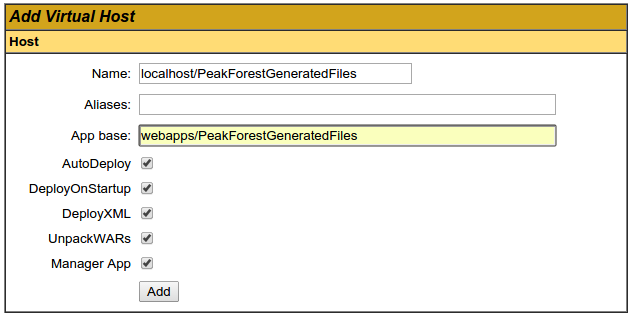
\includegraphics[height=.20\textheight,page=1]{files/images/virtual-host-add.png}
% 	\caption{Create a new virtual host}
% 	\label{createVirtualHost}
% \end{figure}
% 
% \begin{figure}[H]
% 	\centering
% 	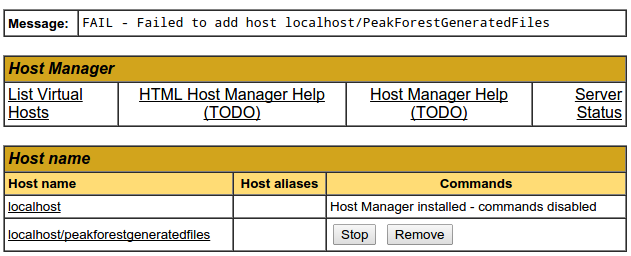
\includegraphics[height=.20\textheight,page=1]{files/images/virtual-host-show.png}
% 	\caption{Check new virtual host creation}
% 	\label{checkCreateVirtualHost}
% \end{figure}
% \egroup		
% 			\caption{Tomcat administration}
% 			\label{tomcatAdministration}
% 		\end{minipage}
% 	}
% \end{figure}
\textbf{Bonus:} By default, Tomcat is running on port 8080.
If you wish to redirect port 80 (default HTTP port) on 8080 follow these instructions:

Create this following script with the command "\texttt{sudo nano /etc/network/if-pre-up.d/iptablesload}" to restore saved IPTABLE.
\begin{lstlisting}[language=bash,caption={/etc/network/if-pre-up.d/iptablesload},frame=bt]
#!/bin/sh
iptables-restore < /etc/iptables.rules
exit 0
\end{lstlisting}

Create this following script with the command "\texttt{sudo nano /etc/network/if-post-down.d/iptablessave}" to save IPTABLE.
\begin{lstlisting}[language=bash,caption={/etc/network/if-post-down.d/iptablessave},frame=bt]
#!/bin/sh
iptables-save -c > /etc/iptables.rules
if [ -f /etc/iptables.downrules ]; then
	iptables-restore < /etc/iptables.downrules
fi
exit 0
\end{lstlisting}

Authorise execution right on these scripts and add IPTABLE rule to redirect port 80 on 8080:
\begin{lstlisting}[language=bash,caption={add execute authorization \& add IPTABLE rule},frame=bt]
# add execute authorization
sudo chmod +x /etc/network/if-post-down.d/iptablessave
sudo chmod +x /etc/network/if-pre-up.d/iptablesload
# reroute 80 port on 8080
sudo iptables -t nat -A PREROUTING -j REDIRECT -p tcp \
	--destination-port 80 --to-ports 8080
\end{lstlisting}

You can now access to the applications hosted on the Tomcat server without the ":8080" between the hostname and the end of the URL.

\textbf{Note:} if you have a system administrator with required skills, you can enable the HTTPS protocol instead of using just HTTP (not secured).

\subsubsection{MySQL - install and create databases}

First install MySQL (if not done in previous step).

\begin{lstlisting}[language=bash,caption={Install MySQL},frame=bt]
# install MySQL if not already done...
sudo apt-get install mysql-server mysql-client libmysqlclient15-dev mysql-common 
# ... set admin password & cie.
# enter MySQL command line tool
mysql -u root -p
\end{lstlisting}

Then execute the following SQL code to create Peak Forest MySQL user and databases. 
Remember the password chose for the MySQL user "peakforest": it will be required later.

\begin{lstlisting}[language=SQL,caption={create MySQL users and databases},frame=bt]
create database peakforest character set utf8;
create database peakforestMeta character set utf8;
create database peakforestExtra character set utf8;
CREATE USER 'peakforest'@'localhost' IDENTIFIED BY 'ENTER_A_STRONG_PASSOWRD';
GRANT ALL PRIVILEGES ON peakforest.* TO 'peakforest'@'localhost';
GRANT ALL PRIVILEGES ON peakforestMeta.* TO 'peakforest'@'localhost';
GRANT ALL PRIVILEGES ON peakforestExtra.* TO 'peakforest'@'localhost';
FLUSH PRIVILEGES;
\end{lstlisting}

\textbf{Note:} feel free to use MariaDB or any fork of MySQL; 
however if you encounter a problem, we may not be able to help you.

\subsubsection{Java - install and set path}

Java JDK is requiered to build Open Babel (see \ref{insallOpenBabel} page \pageref{insallOpenBabel}).

\begin{lstlisting}[language=bash,caption={Install Java and set environment variable },frame=bt]
# install java JDK 
sudo apt-get install openjdk-7-jdk
# add JAVA_HOME as environment variable
echo "export JAVA_HOME=/usr/lib/jvm/java-7-openjdk-amd64/" >> ~/.bashrc
# load new environment variable for current bash session
source  ~/.bashrc
\end{lstlisting}

It is very important when you install Open Babel to have JAVA\_HOME as environment variable. 
Check with a "echo \$JAVA\_HOME" if the variable is setted (must not return a blank result)

\textbf{Note:} you have to install other software / libraries / packages.
The procedure is described below. 

\subsubsection{Paths and directories}

\begin{lstlisting}[language=bash,caption={Paths and directories for Peak Forest},frame=bt]
# Peak Forest files
sudo mkdir /peakforest
sudo mkdir /peakforest/log
sudo mkdir /peakforest/data
sudo mkdir /peakforest/tools
sudo mkdir /peakforest/data/svg
sudo mkdir /peakforest/data/mol
sudo mkdir /peakforest/data/json
sudo mkdir /peakforest/data/cpd-numbered
sudo chown -R tomcat7:tomcat7 /peakforest
# Peak Forest upload files dir
cd /var/lib/tomcat7
sudo mkdir peakforest_uploaded_files
sudo chown tomcat7:tomcat7 peakforest_uploaded_files
\end{lstlisting}

\textbf{Note:} you can set your own path however you must set them in the Peak Forest configuration file (see section TODO page TODO).

\section{Tools dependency installation}

\subsection{Open Babel}
\label{insallOpenBabel}
% intro: open babel is cool
Open Babel\footnote{\url{http://www.jcheminf.com/content/3/1/33}} is a chemical toolbox designed to speak the many languages of chemical data. 
This open and powerful tool is used in Peak Forest to extract all data from a compound (monoisotopic mass, average mass, structures, formula, ...) from the InChI format. 
We chose Ubuntu because most part of third part libraries used by Open Babel can be installed with the aptitude package manager. 
If you use a RedHat or BSD server you must follow the instructions to install Open Babel \href{http://openbabel.org/docs/dev/Installation/install.html}{on their website}.
% open babel

\subsubsection{Install third part libraries in Ubuntu 14.04 - LTS}

The following packages are required to build and install Open Babel on your computer:
\begin{lstlisting}[language=bash,caption={Install packages},frame=bt]
sudo apt-get install gcc cmake wx-common wx2.8-headers libwxbase2.8-dev libxml2 \
	libxml2-dev  zlib1g-dev zlib1g-dev libcairo2-dev  libeigen2-dev \
	build-essential g++ libeigen3-dev python-dev libperl-dev \
	libcurl4-openssl-dev zlib1g-dev checkinstall libwxgtk2.8-dev xterm git
\end{lstlisting}

\subsubsection{Compile Open Babel v2.3.2 with java library}

Open Babel 2.3.2 is used by Peak Forest web-application to gather compound basic data (formula, monoisotopic mass, smiles, ...) form the InChI. 
\begin{lstlisting}[language=bash,caption={Install Open Babel 2.3.2 with java library},frame=bt]
# download Open Babel 2.3.2
cd /tmp/
wget http://sourceforge.net/projects/openbabel/files/openbabel/2.3.2/openbabel-2.3.2.tar.gz/download
mv download download.tar.gz && tar zxf download.tar.gz 
# move source files 
mv openbabel-2.3.2/ ~/ && cd ~/
mkdir build_openbabel_2.3.2 && cd build_openbabel_2.3.2
# build Open Babel
cmake ../openbabel-2.3.2 -DJAVA_BINDINGS=ON
make -j2
sudo make install
\end{lstlisting}

Edit Tomcat service script with the \texttt{sudo nano /etc/init.d/tomcat7} command. 
Be careful to not edit other sections of the script. 
\begin{lstlisting}[language=bash,caption={Tomcat service script},frame=bt]
# ...
if [ `id -u` -ne 0 ]; then
        echo "You need root privileges to run this script"
        exit 1
fi

# ADD THIS SECTION - DO NOT EDIT THE CODE BEFORE
export CATALINA_OPTS="-Xms512M -Xmx1024M -Djava.library.path=/usr/local/lib"
# END ADD THIS SECTION - DO NOT EDIT THE CODE AFTER

# Make sure tomcat is started with system locale
if [ -r /etc/default/locale ]; then
# ...
\end{lstlisting}

\subsubsection{Compile Open Babel command line call with a specific path}

This version of Open Babel is used to generate the molecules mol files, svg images and compute molecules logP property.
\begin{lstlisting}[language=bash,caption={Install a specific version of Open Babel in a specific directory},frame=bt]
# download Open Babel 40bc0f10
cd ~ && git clone git://github.com/openbabel/openbabel.git
cd openbabel && git checkout 40bc0f105c3d3dc7f189cd6d54ddfef6f5452dbf
# move source files
cd ~ && mv openbabel openbabel-40bc0f10 
mkdir build_openbabel_40bc0f10 && cd build_openbabel_40bc0f10/
# build Open Babel 
cmake ../openbabel-40bc0f10 -DCMAKE_INSTALL_PREFIX=/usr/local/bin/openbabel-40bc0f10
make -j2 # (may take a while... Fancy a coffee?)
sudo make install
\end{lstlisting}

\textbf{Note:} This guide / tutorial was created on October 2015. 
If a newer release of Open Babel is available please contact us and we will test if this section is still necessary.

%\section{Tomcat \& database}
\subsection{Peak Matching tools}

\subsubsection{NMR PeakMatching}

This peakmatching tool is powered by "NMR PeakMatching 1.0" (\textcopyright INRA UMR 1332 - MetaboHUB). 
For more informations, please visit \href{http://www.bordeaux.inra.fr/pmb/PM/webapp}{NMR PeakMatching} website.

\subsubsection{BiH - Bank in-House}

This peakmatching tool is powered by "Bank in House" (\textcopyright INRA UMR 1019 - F.L.A.M.E. / W4M). 
To install it, just clone the Git repository in "/peakforest/tool" directory. 
Please checkout the tag "release\_2015.11.25" (no test were run on the other BiH releases).

\begin{lstlisting}[language=bash,caption={Install BiH tool},frame=bt]
# Peak Forest files
cd /peakforest/tools
git clone https://pfemw3.clermont.inra.fr/gitlab/dev-team/tool-bank_inhouse.git
cd tool-bank_inhouse && git fetch && git checkout tags/release_2015.11.25
# install BiH perl libraries
sudo cpan install LWP::Simple module
sudo cpan install SOAP::Lite module
sudo cpan install Text::CSV module
\end{lstlisting}

For more information about BiH tool, please refer to \href{http://galaxy.workflow4metabolomics.org/root?tool_id=toolshed4metabolomics.sb-roscoff.fr:9009/repos/pfem/bank_inhouse/bank_inhouse/1.0.0}{workflow4metabolomics.org} website.

\subsubsection{PeakMatching CEA}

TODO

\section{Downloads \& Copyright}

\subsection{MetaboHUB downloads}

\subsection{License}

\subsection{Contact}

\newpage
\newpage

%%% bibliographie %%%

%\bibliographystyle{unsrt}
%\bibliography{files/biblio}

\end{document}
